% Created 2023-07-12 Wed 16:25
% Intended LaTeX compiler: pdflatex

% =================================BASE====================================%
\documentclass[10pt]{article}
\usepackage[left=2cm,right=2cm,top=2cm,bottom=2cm]{geometry} % Marges
%\usepackage{libertine}
%\usepackage{libertinust1math}
\usepackage[T1]{fontenc} % Nécessaire avec FrenchBabel
\usepackage[utf8]{inputenc} % Important pour symboles Francophones, é,à,etc

\usepackage{lmodern}
\renewcommand{\familydefault}{cmr} % La meilleure police (CMU Serif Roman) (Je me suis battu).

\usepackage{natbib} % Bibliographie
\bibliographystyle{abbrvnat}



\usepackage{amsmath, amssymb, amsthm} % Symb. math. (Mathmode+Textmode) + Beaux théorèmes.

\usepackage{mathtools,cancel} % Utilisation de boîtes \boxed{} + \cancelto{}{}
\usepackage{graphicx, wrapfig} % Géstion des figures.
\usepackage{hyperref} % Permettre l'utilisation d'hyperliens.
\usepackage{color} % Permettre l'utilisation des couleurs.
\usepackage[dvipsnames]{xcolor} % Couleurs avancées.
\usepackage{titling} % Donne accès à \theauthor, \thetitle, \thedate

% >>> Physique >>>
\usepackage{physics} % Meilleur package pour physicien. 
\usepackage{pxfonts} % Rajoute PLEIN de symboles mathématiques, dont les intégrales doubles et triples
% <<< Physique <<<

\usepackage{lipsum} % For fun
\usepackage{tikz} % Realisation de figures TIKZ.
\usepackage{empheq} % Boite autour de MULTIPLE équations

\usepackage[french]{babel} % Environnements en Français.
% ==============================BASE-(END)=================================%



% ================================SETTINGS=================================%
% Pas d'indentation en début de paragraphe :
\setlength\parindent{0pt} 

% Couleurs de hyperliens :
\definecolor{mypink}{RGB}{147, 0, 255}
\hypersetup{colorlinks, urlcolor=mypink, citecolor=mypink, linkcolor=mypink}

% Numéros d'équations suivent les sections :
\numberwithin{equation}{section} 

% Les « captions » sont en italique et largeur limitée
\usepackage[textfont = it]{caption} 
\captionsetup[wrapfigure]{margin=0.5cm}


% Retirer le l'écriture en gras dans la table des matières
\usepackage{tocloft}
\renewcommand{\cftsecfont}{\normalfont}
\renewcommand{\cftsecpagefont}{\normalfont}

% Change bullet style
\usepackage{pifont}
\usepackage{enumitem}
\setlist[itemize,1]{label=\ding{224}}
% ================================SETTINGS=================================%



% ==============================NEWCOMMANDS================================%
% Degrés Celsius :
\newcommand{\celsius}{${}^\circ$ C} % \degrée Celsius : Pas mal plus simple qu'utilise le package gensymb qui plante avec tout...

% Vecteurs de base :
\newcommand{\nvf}{\vb{\hat{n}}}
\newcommand{\ivf}{\vb{\hat{i}}}
\newcommand{\jvf}{\vb{\hat{j}}}
\newcommand{\kvf}{\vb{\hat{k}}}

\newcommand{\uu}{\vb*{u}}
\newcommand{\vv}{\vb*{v}}

% Boîte vide pour ajuster les underbrace
\newcommand{\bigno}{\vphantom{\qty(\frac{d}{q})}}
\newcommand{\pt}{\hspace{1pt}}

% Physics empty spaces 
\newcommand{\typical}{\vphantom{A}}
\newcommand{\tall}{\vphantom{A^{x^x}_p}}
\newcommand{\grande}{\vphantom{\frac{1}{xx}}}
\newcommand{\venti}{\vphantom{\sum_x^x}}

% Moyenne numérique entre deux points de grilles. 
\newcommand{\xmean}[1]{\overline{#1}^x}
\newcommand{\ymean}[1]{\overline{#1}^y}
\newcommand{\zmean}[1]{\overline{#1}^z}
\newcommand{\xymean}[1]{\overline{#1}^{xy}}

% Tilde over psi
\newcommand{\tpsi}{\tilde{\psi}}

% Nota Bene env :
\newcommand{\nb}{\textbf{N.B.}\hspace{4pt}}
   
% ==============================NEWCOMMANDS================================%



% ==============================PAGE-TITRE=================================%
% Titlepage 
\newcommand{\mytitlepage}{
\begin{titlepage}
\begin{center}
{\Large Contrat Été 2023 \par}
\vspace{2cm}
{\Large \MakeUppercase{\thetitle} \par}
\vspace{2cm}
RÉALISÉ DANS LE CADRE\\ D'UN PROJET POUR \par
\vspace{2cm}
{\Large ISMER--UQAR \par}
\vspace{2cm}
{\thedate}
\end{center}
\vfill
Rédaction \\
{\theauthor}\\
\url{charles-edouard.lizotte@uqar.ca}\\
ISMER-UQAR
\end{titlepage}
}
% ==============================PAGE-TITRE=================================%



% =================================ENTÊTE==================================%
\usepackage{fancyhdr}
\pagestyle{fancy}
\setlength{\headheight}{13pt}
\renewcommand{\headrulewidth}{1.3pt} % Ligne horizontale en haut

\fancyhead[R]{\textit{\thetitle}}
\fancyhead[L]{\ \thepage}
\fancyfoot[R]{\textit{\theauthor}}
\fancyfoot[L]{}
\fancyfoot[C]{} 
% =================================ENTÊTE==================================%
\author{Charles-Édouard Lizotte}
\date{07/07/2023}
\title{Carnet de bord, Université McGill}
\hypersetup{
 pdfauthor={Charles-Édouard Lizotte},
 pdftitle={Carnet de bord, Université McGill},
 pdfkeywords={},
 pdfsubject={},
 pdfcreator={Emacs 27.1 (Org mode 9.6.5)}, 
 pdflang={French}}
\begin{document}

\mytitlepage
\tableofcontents\newpage



\section{{\bfseries\sffamily DONE} Présentation des résultats de maîtrise}
\label{sec:org20ce7b2}
Ce mercredi 5 juillet, le groupe à David m'avait proposé de réaliser une présentation sur mon projet de maîtrise (de 2019 à 2022).
Personnellement, je trouvais que c'était une bonne occasion de me remettre à niveau sur ce qui avait été réalisé, tout en revisitant certains résultats intéressants datant du début du projet.
Aussi, ça m'a permis de faire une présentation en Anglais, ce qui n'avait pas vraiment été pertinent jusqu'à maintenant.
Donc, c'est pourquoi lundi et mardi, j'ai passé beaucoup de temps à remettre à jour ce vieux \emph{beamer} réalisé pour ma présentation des résultats en 2021.
À l'époque, je n'avais tout simplement pas de résultats à afficher, donc j'ai pu additionner quelques figures intéressantes à la présentation et réparer des figures Tikz en passant.
Je crois que le résultat de mercredi a été satisfaisant.
J'ai beaucoup d'aisance à parler du projet, des concepts sous-jacents et des objectifs.
J'aimerais bien ajouter une partie historique sur les vagues parlant de vieux articles ayant mené à des découvertes intéressantes dans le dossier.
Je pense que ça sera une objectif pour une autre présentation.\bigskip

Entre autres, un article de Charnok des années 50 sur le profil logarithmique, les découvertes de Miles et Philipps sur le décalage entre la pression et la crète de vagues, soit le méchanisme d'évolution des vagues.
Aussi, ça me permettrait de revisiter certains concepts, comme le calcul menant à la dérive de Stokes et le fameux \emph{Garden-Sprinkler effect}.
Bref, je met ça ici pour m'en souvenir.

\section{Toujours des problèmes dans la divergence du courant barotrope}
\label{sec:org644b740}

\subsection{Diagnostique}
\label{sec:org5a3bfea}
Encore et toujours, nous avons des problèmes avec la divergence du courant barotrope, comme démontré dans le dernier rapport.
Certaines informations pertinentes :
\begin{itemize}
\item La divergence barotrope n'est pas nulle : Des «points» apparaissent dans la divergence et croient de manière linéaire avec le temps. C'est un problème car ça va créer de l'erreur numérique à long terme. L'erreur est de l'ordre de 1e-11 quand la divergence de chaque couche est autour de 1e-9 (voir figure \ref{fig:orgda9f588}).
\item La divergence du RHS barotrope, soit la quantité qui sort directement de MUDPACK est de 1e-19. C'est donc énormément plus petit. On pourrait pas mal dire que c'est de l'ordre de l'erreur numérique.
\end{itemize}

\begin{figure}[htbp]
\centering
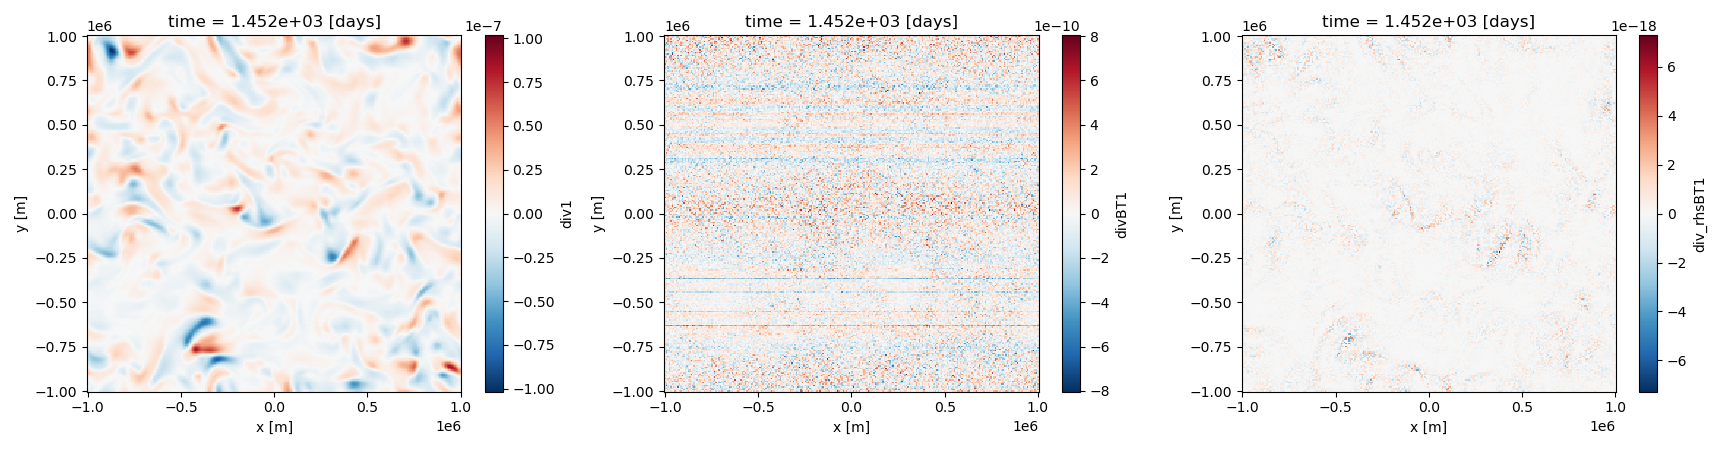
\includegraphics[width=.9\linewidth]{figures/debuggage/2023_07_010_3div1.png}
\caption{\label{fig:orgda9f588}Figure illustrant trois quantités reliées à la divergence au dernier pas de temps -- autour de 1450 jours. En ordre : la divergence de la première couche; la divergence barotrope du courant pour toutes les couches; la divergence du RHS du modèle.}
\end{figure}

Avant le \emph{spin up}, les erreurs ont une forme légèrement différentes, mais le résultat est le même (voir figure \ref{fig:org4d9389e}).

\begin{figure}[htbp]
\centering
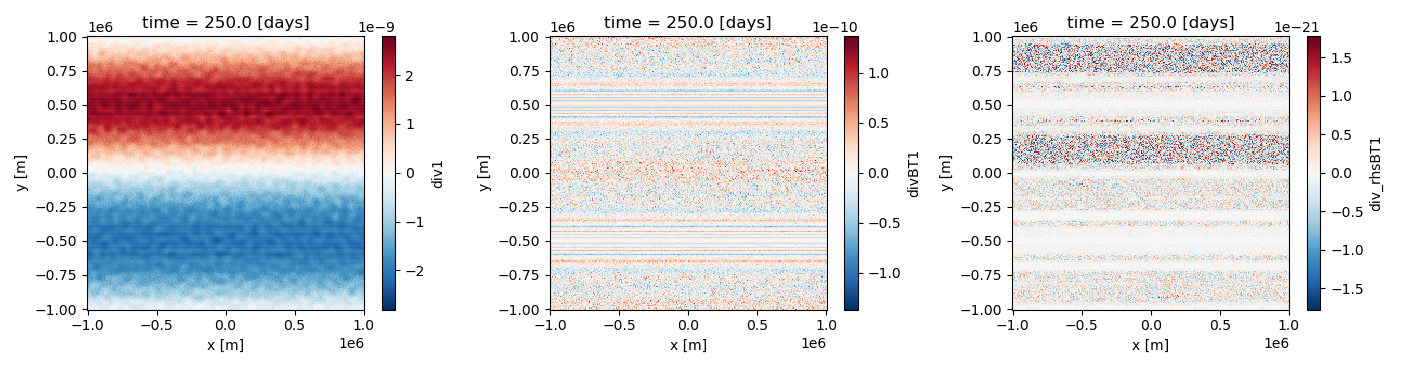
\includegraphics[width=.9\linewidth]{figures/debuggage/2023_07_010_3div1_t250.png}
\caption{\label{fig:org4d9389e}Figure illustrant trois quantités reliées à la divergence au jour 250. En ordre : la divergence de la première couche; la divergence barotrope du courant pour toutes les couches; la divergence du RHS du modèle.}
\end{figure}


\subsection{Hypothèse}
\label{sec:org4706008}
Donc mon hypothèse est que ça se cache dans la partie barocline et non de MUDPACK.
Voici l'argument que je fais :
\begin{itemize}
\item La partie barotrope du \emph{RHS} provient d'une correction de la fonction de courant barotrope (\(\psi_{BT}\)), donc par définition sa divergence \textbf{doit être nulle}. Ceci est aussi démontrable à l'aide des \emph{output}.
\item La partie barocline du RHS est mise à jour sans avoir été corrigée pour être adivergente.
Donc, il peut y avoir une partie divergente qui se cache dans cette dernière et ce truc-là grandit à chaque pas de temps.
\end{itemize}

Donc, au final on n'a pas de méchanisme de rappel qui vient tuer la partie divergente du flow, contrairement au modèle solutionné par FFTW.
Il faudrait trouver une solution.
Après une rencontre ce vendredi avec David et LP, on propose cordialement de retirer la partie divergente à tous les dix pas de temps, ce qui devrait demander une autre run de MUDPACK, mais le coût numérique est très faible.

\subsection{Solution}
\label{sec:org46abf7b}

À tous les 100 pas de temps, on pourrait retirer la partie non-divergente de notre écoulement.
Dans ce cas, on appliquerait donc une correction à notre écoulement barotrope.
En premier lieu, il est extrêmement simple à prouver la moyenne barotrope des vorticités et égale au rotationnel du courant barotrope, soit
\begin{equation}
\label{eq:org498b92d}
   \zeta_{BT} = \qty(\frac{1}{H})\sum_k^n h_k\zeta_k = \qty(\frac{1}{H})\sum_k^n h_k\pt \kvf \cdot \curl{\uu_k} = \qty(\frac{ \kvf}{H})\cdot\sum_k^n\curl(h_k\uu_k) = \kvf\cdot\curl(\frac{1}{H}\sum_k^n h_k\uu_k) = \kvf\cdot\curl{\uu_{BT}},
\end{equation}
car le produit vectoriel est un opérateur linéaire (\ref{eq:org498b92d}).
Il existe donc deux méthodes pour trouver la vorticités barotrope.\bigskip

Le processus pour corriger notre écoulement est simple, on sait que
\begin{equation}
\label{eq:org490c56c}
   \laplacian(\psi_{BT}) = \zeta_{BT}.
\end{equation}
Comme à l'habitude, notre écoulement est divisé en deux parties, soit barotropes (voir \ref{eq:org498b92d}) et baroclines ,
\begin{equation}
   \uu = \uu_{BT} + \uu_{BC}.
\end{equation}
Une fois \ref{eq:org490c56c} solvé, on retrouve notre courant barotrope corrigé (\(\uu_{BT}'\)) à l'aide de
\begin{equation}
   \uu_{BT}' = \curl(k\psi_{BT}),
\end{equation}
et l'on retroue le courant à l'aide de
\begin{equation}
   \uu = \uu_{BT}' + \uu_{BC}.
\end{equation}


\subsection{Résultats}
\label{sec:orga89f177}
Ça ne parche pas vu qu'on est en périodique.
Voici la nature du problème : les frontières sont périodiques, \emph{MUDPACK} essaie donc de relier les dérivées aux frontières sans considération de la constante d'intégration.
Finalement, la solution relative par rapport à la constante d'intégration devient minuscule et on perd de plus en plus de précision.
On se retrouve alors dans une \emph{feedback loop} où le système est mal résolue, ce qui vient exacerber les instabilités numériques créées par l'erreur numérique relative, car les erreur nécessite une dérivée de plus en plus forte, ce qui fait aussi monter la constante d'intégration, etc.
Pour résumer, voici un passage de la documentation de MUDPACK :

\begin{quote}
\emph{« [If] the continuous elliptic pde is singular.  this means the boundary conditions are periodic or pure derivative at all boundaries and ce(x,y) = 0.0 for all x,y.  a solution is still attempted but convergence may not occur due to ill-conditioning of the linear system coming from the discretization.»}
\end{quote}

Donc, on embarque sur les murs au plus vite.

\section{{\bfseries\sffamily TODO} Les murs}
\label{sec:org3ceb940}
Ok, il faut absolument embarquer sur les murs avant que je parte en vacance.

\subsection{{\bfseries\sffamily TODO} Nombre de points}
\label{sec:orgd745e8d}

\begin{wrapfigure}{r}{0.4\textwidth}
\vspace{-\baselineskip}
\begin{center}
\begin{tikzpicture}
%
\foreach \i in {0,1,2,3}
{\foreach \j in {-1,0,1,2,3}
{\draw [thick, red!30] (\i,\j+1) -- (\i,\j) ;
 \draw [thick,blue!30] (\j,\i) -- (\j+1,\i) ;}}
%
\foreach \i in {0,1,2,3}
{\foreach \j in {-1,0,1,2,3}
{\draw [-latex,thin,red!30 ] (\i,0.5+\j) -- (\i+0.15,0.5+\j);
 \draw [-latex,thin,blue!30] (0.5+\j,\i) -- (0.5+\j,\i+0.15);}}
%
\foreach \i in {0,1,2,3,4}
{\foreach \j in {0,1,2,3,4}
{\fill[fill=black ] (\i-0.53,\j-0.53) rectangle (\i-0.47,\j-0.47);}}
%
\draw [ultra thin,gray] (0,0) rectangle (3,3);
%
\draw[> = latex, arrows = {|<->|}, thin] (0,4.5) -- (3,4.5);
\draw (1.5,4.5) node [above] {nx};
\draw[> = latex, arrows = {|<->|}, thin] (-1.5,0) -- (-1.5,3);
\draw (-1.5,1.5) node [left] {ny};
%
\foreach \i in {0,1,2,3}
\foreach \j in {0,1,2,3}
{{\filldraw [black!85] (\i,\j) circle (0.8pt);}}
\end{tikzpicture}
\end{center}
\caption{\label{orgd1e6286}Grille  avec frontières fixes.}
\end{wrapfigure}


Avant tout, on change complétement la définition de notre grille.
Précédemment, on utilisait toujours une grille de taille \((nx+1)\times(ny+1)\), mais ceci est en mesure de changer avec des frontières fixes.
En premier lieu, la condition \emph{free slip} nécéssite l'ajout de points fantomes sur les axes parallèles, de sorte que
\begin{align}
&&   \eval{\pdv{v}{x}\pt}_\text{i=1,nx} = \ 0, && \eval{\pdv{u}{y}\pt}_\text{j=1,ny} =\ 0, &&
\end{align}

La même condition s'applique aussi sur l'épaisseur des couches, de sorte que
\begin{align}
   &&   \eval{\pdv{h}{x}\pt}_\text{i=1,nx} = \ 0, && \eval{\pdv{h}{y}\pt}_\text{j=1,ny} =\ 0, &&
\end{align}

Pour être plus précis les dimensions seront données par
\begin{itemize}
\item u(nx,0:ny+1)
\item v(0:nx+1,ny)
\item eta(0:nx+1,0:ny+1)
\item zeta(nx,ny)
\end{itemize}

\subsection{Condition no-normal flow}
\label{sec:org0c92980}
La condition \emph{no-normal flow} est tout simplement donnée par
\begin{align}
   && u\pt(\pt:\pt,1) = u\pt(:\pt,ny) = 0, && v\pt(1,:\pt) = v\pt(nx,:\pt) = 0. &&
\end{align}


\subsection{Condition free slip}
\label{sec:org87d6040}
Avec notre nouvelle définition de grille, la condition \emph{free slip} est tout simplement donnée par
\begin{align}
    && u\pt(\pt0,:) = u\pt(1,:); && u\pt(nx+1,:) = u\pt(nx,:) && \\
    && v\pt(\pt:\pt,0) = v\pt(:,1); && v\pt(:\pt,ny+1) = v\pt(\pt:,ny) &&
\end{align}
\end{document}